%Beschreibung der Implementierung der Darstellungen auf den Displays
Die Komponente \texttt{LED-Panels} empfängt Daten der Panelinformationen von der Komponente \texttt{Flüssigkeitssimulation} und beleuchtet die Panels entsprechend dieser Daten. Die Anzahl der Wasserteilchen pro Pixel dient als Intensität der blauen Farbe einer LED. Als Referenz diente das Projekt \cite{rgbLedMatrix} in Adafruit.

\subsection{Hardware}
Der RGB-Würfel wird aus sechs 32$\times$32 RGB Matrix LED-Panelen aufgebaut. Zum Betrieb eines Panels $2A$ an Strom benötigt. Die 6 Panele werden durch eine Stromversorgung aktiviert. Auf der Rückseite eines jeden Panels befinden sich ein Eingangs- und ein Ausgangsport mit jeweils 16 Pins. Diese sind für die Farbinformation R1, G1, B1, R2, G2, B2, die Adresssignale A, B, C, D und die Steuersignale CLK (Takt), OE (Output Enable), LAT (Latch), und 3 GNDs. Ein Panel wird über ein 16-Leitungs Kabel direkt mit dem Board verbunden (siehe Abbildung \ref{fig:led:plug}), die restlichen fünf Panels werden nacheinander mit Flachbandkabel verbunden (Ausgangsport des einen Panels wird mit dem Eingangsport eines Nächsten verbunden), welches Daisy-Chain genannt wird (Abbildung \ref{fig:led:chain}). 

\begin{figure}[h!]
	\centering
	\begin{minipage}[t]{0.45\linewidth}
	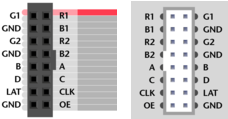
\includegraphics[width=.9\linewidth]{led/led_matrix_plug.png}
	\caption{Port mit Beschriftung von Buchse bzw. Flachbandkabel}
	\label{fig:led:plug}
	\source{Quelle: \cite{rgbLedMatrix}(Connecting with Jumper Wires)}
	\end{minipage}
	\hspace{0.05\linewidth}
	\begin{minipage}[t]{0.45\linewidth}
	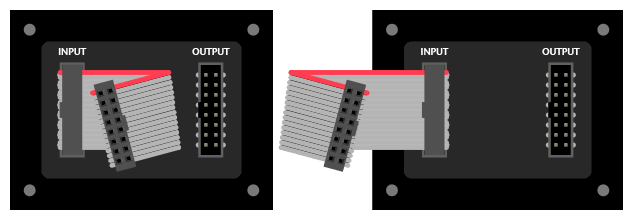
\includegraphics[width=.9\linewidth]{led/led_matrix_ribbon}
	\caption{Panels per Daisy-Chain}
	\label{fig:led:chain}
	\source{Quelle: \cite{rgbLedMatrix}(Connecting with Jumper Wires)}
	\end{minipage}
\end{figure}

Die Eingänge der RGB-, Adress- und Steuersignale des ersten Panels werden mit GPIO (General Purpose Input Output) Pins auf dem Board verbunden, Port 2.0 bis 2.5 bzw. Port 3.0 bis 3.6. Als Default-Einstellung vom Hersteller sind Port 2.0 bis 2.7 direkt mit den LEDs vom Board verbunden. Daher muss der Jumper \texttt{LED} entnommen werden, um diese Pins für die Anzeige anzuwenden. Abbildung \ref{fig:assembly:dice} stellt den gesamten Aufbau der Komponente Würfel dar.

\begin{figure}
	\centering
	\includegraphics[width=0.95\linewidth]{example-image}
	\caption[Aufbau von sechs 32$\times$32 RGB Matrix LED-Panels]{Aufbau von sechs 32$\times$32 RGB Matrix LED-Panels. }
	\label{fig:assembly:dice}
\end{figure}

\subsection{Konfiguration und Mechanismus einer Anzeige}
Hier wird beschrieben, wie ein aus 32 Zeilen $\times$ 32 Spalten insgesamt 1024 LEDs bestehendes Panel gesteuert wird. Die  RGB-Signale R1, G1 und B1 sowie R2, G2 und B2 bilden die LED-Farbe eines Pixels des oberen bzw. unteren Teils des Panels. Das Panel installiert 32-bit Schieberegister, womit die kompletten Farbdaten einer Zeile gespeichert werden. Das Verschieben geschieht durch das Taktsignal. Es lässt somit zwei Zeilen gleichzeitig anzeigen. Dies soll in schneller als 20 $ms$ geschehen, damit menschliche Augen einen Anzeigewechsel nicht merken und diesen als ein Standbild erfassen. Diese zwei Zeilen sind erste und 17. Zeile, zweite und 18. Zeile, ..., und 16. und 32. Zeile, die durch eine Adresse festgelegt werden, welche von den Adresssignale A, B, C und D definiert wird.\\

\emph{<Schritte>}
\begin{enumerate}
	\item Setzen alle Pins auf \texttt{Low} (anfang)
	\item \texttt{R1,G1,B1,R2,G2,B2} Pins auf \texttt{High/Low} setzen
	\item \texttt{CLK} Pin auf \texttt{High} setzen
	\item \texttt{CLK} Pin auf \texttt{Low} setzen \\
	(Farbinformation wird in den Schiebregister geladen.)
	\item Schritte 2-4 für alle Spalten wiederholen
	\item Mit Adresspins \texttt{ABCD} eine gezielte Zeile (gleichzeitig von der oberen und unteren Hälfte) auswählen
	\item \texttt{OE} Pin auf \texttt{High} setzen
	\item \texttt{LAT} Pin auf \texttt{High} setzen (erleuchtet LED)
	\item \texttt{LAT} Pin auf \texttt{Low} setzen
	\item \texttt{OE} Pin auf \texttt{Low} setzen
	\item Zurück zum Schritt 1
\end{enumerate}

Werden Panels verkettet, werden die Signale seriell weiter geleitet und die Farbinformation muss daher bis zum letzten Spalten reingeschoben werden. Das bedeutet, die verketteten Panels können letztendlich als ein langes Panel betrachtet werden.

Als nächstes soll die Darstellung der Farbintensität betrachtet werden. Das Display besitzt keine PWM-Funktionalität und lässt ein LED nur \texttt{An} oder \texttt{Aus} schalten. Um unterschiedliche Blaufarben zu realisieren, wird die Methode von Binary Code Manipulation verwendet (siehe XXX zum Detail). 

\subsection{Software}
 Zur Anwendung GPIO Pins müssen die folgenden Schritte (Quelltext \ref{code:ledinit}) durchgeführt werden.
\begin{lstlisting}[language={c}, caption={Initialisierung von GPIO als Output}, label={code:ledinit}]
void led_init(void)
{
    PINSEL10 = 0;    ///< Disable ETM interface, enable LEDs (turn all LEDs on)
    PINSEL4 = 0;     ///< Set function GPIO on port 2
    FIO2DIR  = 0xFF; ///< P2.0..7 defined as output
    FIO2MASK = 0;    ///< Enable write, set, clear, and read to R/W port 2
}

void led32x32_init(void)
{
    led_init();

    // Set port 3
    PINSEL6 = 0;     ///< Set function GPIO on port 3.0..5
    FIO3DIR = 0xFF;  ///< P3.0..7 defined as output
    FIO3MASK = 0;    ///< Enable write, set, clear, and read to R/W port 3
}
\end{lstlisting}

Zur Steuerung der Signale werden die Unterfunktionen (Quelltext \ref{code:ctrlsig}) geschrieben. Durch \texttt{FIO2SET} und \texttt{FIO2CLR} Register (analog zu \texttt{FIO3}) wird der Ausgang eines Pins auf \texttt{1} bzw. auf \texttt{0} gesetzt. Diese Grundfunktionen werden in den jeweiligen Funktionen (RGB-Signale, Adresssignale und Steuersignale) aufgerufen.

\begin{lstlisting}[language={c}, caption={Funktionen zur Steuerung der Signale.}, label={code:ctrlsig}]
#define LED32X32_RGBPIN_SETTER   FIO2SET
#define LED32X32_RGBPIN_CLEANER  FIO2CLR
#define LED32X32_CTRLPIN_SETTER  FIO3SET
#define LED32X32_CTRLPIN_CLEANER FIO3CLR

static inline void lp32x32_setCtrlPin(int pin)
{
    LED32X32_CTRLPIN_SETTER |= (1 << pin);
}
static inline void lp32x32_clearCtrlPin(int pin)
{
    LED32X32_CTRLPIN_CLEANER |= (1 << pin);
}
static inline void lp32x32_setRgbPin(int pin)
{
    LED32X32_RGBPIN_SETTER |= (1 << pin);
}
static inline void lp32x32_clearRgbPin(int pin)
{
    LED32X32_RGBPIN_CLEANER |= (1 << pin);
}
\end{lstlisting}

Überlagerung mehreren Schichten zur Realisierung einer 24-bit Farbe wird dadurch implementiert, dass der Zyklus der 1-zeiligen Anzeige entsprechend der Schichtenanzahl wiederholt wird. Dazu benötigt das System einen noch schnelleren Takt. Quelltext \ref{code:ledmain} zeigt die Kernfunktion dieses Moduls.

\begin{lstlisting}[language={c}, caption={Schritte von Panel-Anzeige}, label={code:ledmain}]

void lp32x32_refresh_chain_24bit_rgb(panel_t panels[CHAIN_LEN])
{
    static uint8_t row = 0;
    static uint8_t color_bit = 0;
    uint8_t col;
    uint8_t layer;
    uint8_t panelIndex = 0;
    uint32_t upperPixel = 0;
    uint32_t bottomPixel = 0;

    for(layer = 0; layer < 1; ++layer)
    {
        for(col = 0; col < (COL_NUM * CHAIN_LEN); ++col)
        {
            panelIndex = col / COL_NUM;
            upperPixel = panels[panelIndex][row][col - COL_NUM * panelIndex].particle_count;
            bottomPixel = panels[panelIndex][row + ROW_NUM / 2][col - COL_NUM * panelIndex].particle_count;
            
            lp32x32_setUpperPixelInfo((/*red=  */((upperPixel  & LED32X32_RGB24_R_MASK) >> 16) & (0x01 << color_bit)), 
                                       (/*green=*/((upperPixel  & LED32X32_RGB24_G_MASK) >>  8) & (0x01 << color_bit)),
                                       (/*blue= */((upperPixel  & LED32X32_RGB24_B_MASK)      ) & (0x01 << color_bit)));
            lp32x32_setBottomPixelInfo((/*red=  */((bottomPixel & LED32X32_RGB24_R_MASK) >> 16) & (0x01 << color_bit)), 
                                       (/*green=*/((bottomPixel & LED32X32_RGB24_G_MASK) >>  8) & (0x01 << color_bit)),
                                       (/*blue= */((bottomPixel & LED32X32_RGB24_B_MASK)      ) & (0x01 << color_bit)));

            lp32x32_clock(); ///< Shift RGB information of each pixel to horizontal direction
        }

        lp32x32_setRow(row);
        lp32x32_setCtrlPin(LED32X32_PIN_OE);
        lp32x32_latch();
        lp32x32_clearCtrlPin(LED32X32_PIN_OE);
    }
    ++row;
    if(row >= (ROW_NUM/2))
    {
        row = 0;
        ++color_bit;
    }
    if(color_bit >= 8)
    {
        color_bit = 0;
    }
}
\end{lstlisting}
